\section{Energy scale calibration}
\label{sec:energy_scan}

\subsection{Resolution Scans}
\label{sec:resolution_scans}
As the signal from the detector is rather weak, the detector is connected to an
amplifying circuit as described in Sect.~\ref{sec:calibration:set-up}. However
there is a trade-off associated with this procedure as amplification also
applies to noise in the detector. In order to increase the signal strength the
voltage applied to the detector can be increased which in turn increases the
amount of signal electrons and leads to a stronger output signal. Along with
this comes though an increased probability for spontaneous discharges along
impurities and dirt remaining in the detector despite extensive cleaning
procedures as described in Sect.~\ref{sec:construction}.

As the two possibilities for varying the output signal strength are associated
with independent increases of noise and accordingly reduction of resolution we
are performing resolution scans for the two samples we are interested in
measuring: Americium and Iron.

In order to reliably determine the resolution a Gaussian is fitted to the sample
peak previously identified in the MCA spectrum. We look
at the variable peak width divided by the peak position in order to determine
the resolution of our peak. For the peak width we are using the full-width
half-maximum (FWHM) value. As secondary decays will affect especially the lower
end of the decay Gaussian shape we are defining regions of interest (ROI) in which the Gaussian
is fitted.

The spectra obtained for americium (Fig.~\ref{fig:scan:americium}) and iron
(Fig.~\ref{fig:scan:iron}) are presented in App.~\ref{app:resolution-scans} for different gains and voltages.
A Gaussian is fitted to the marked ROI (blue lines) and the obtained channel number as well as
full-width half-maximum (FWHM) in channels are denoted in each figure.

The obtained parameters from the fit are plotted in Figs.~\ref{fig:resolution:americium} and \ref{fig:resolution:iron} for americium and
iron respectively. The uncertainties are propagated from the fit. Additionally to the
total uncertainty on the FWHM, a \SI{10}{\percent} systematic
uncertainty was added due to the dependency on choosing the corresponding ROI.

\begin{figure*}[htbp]
  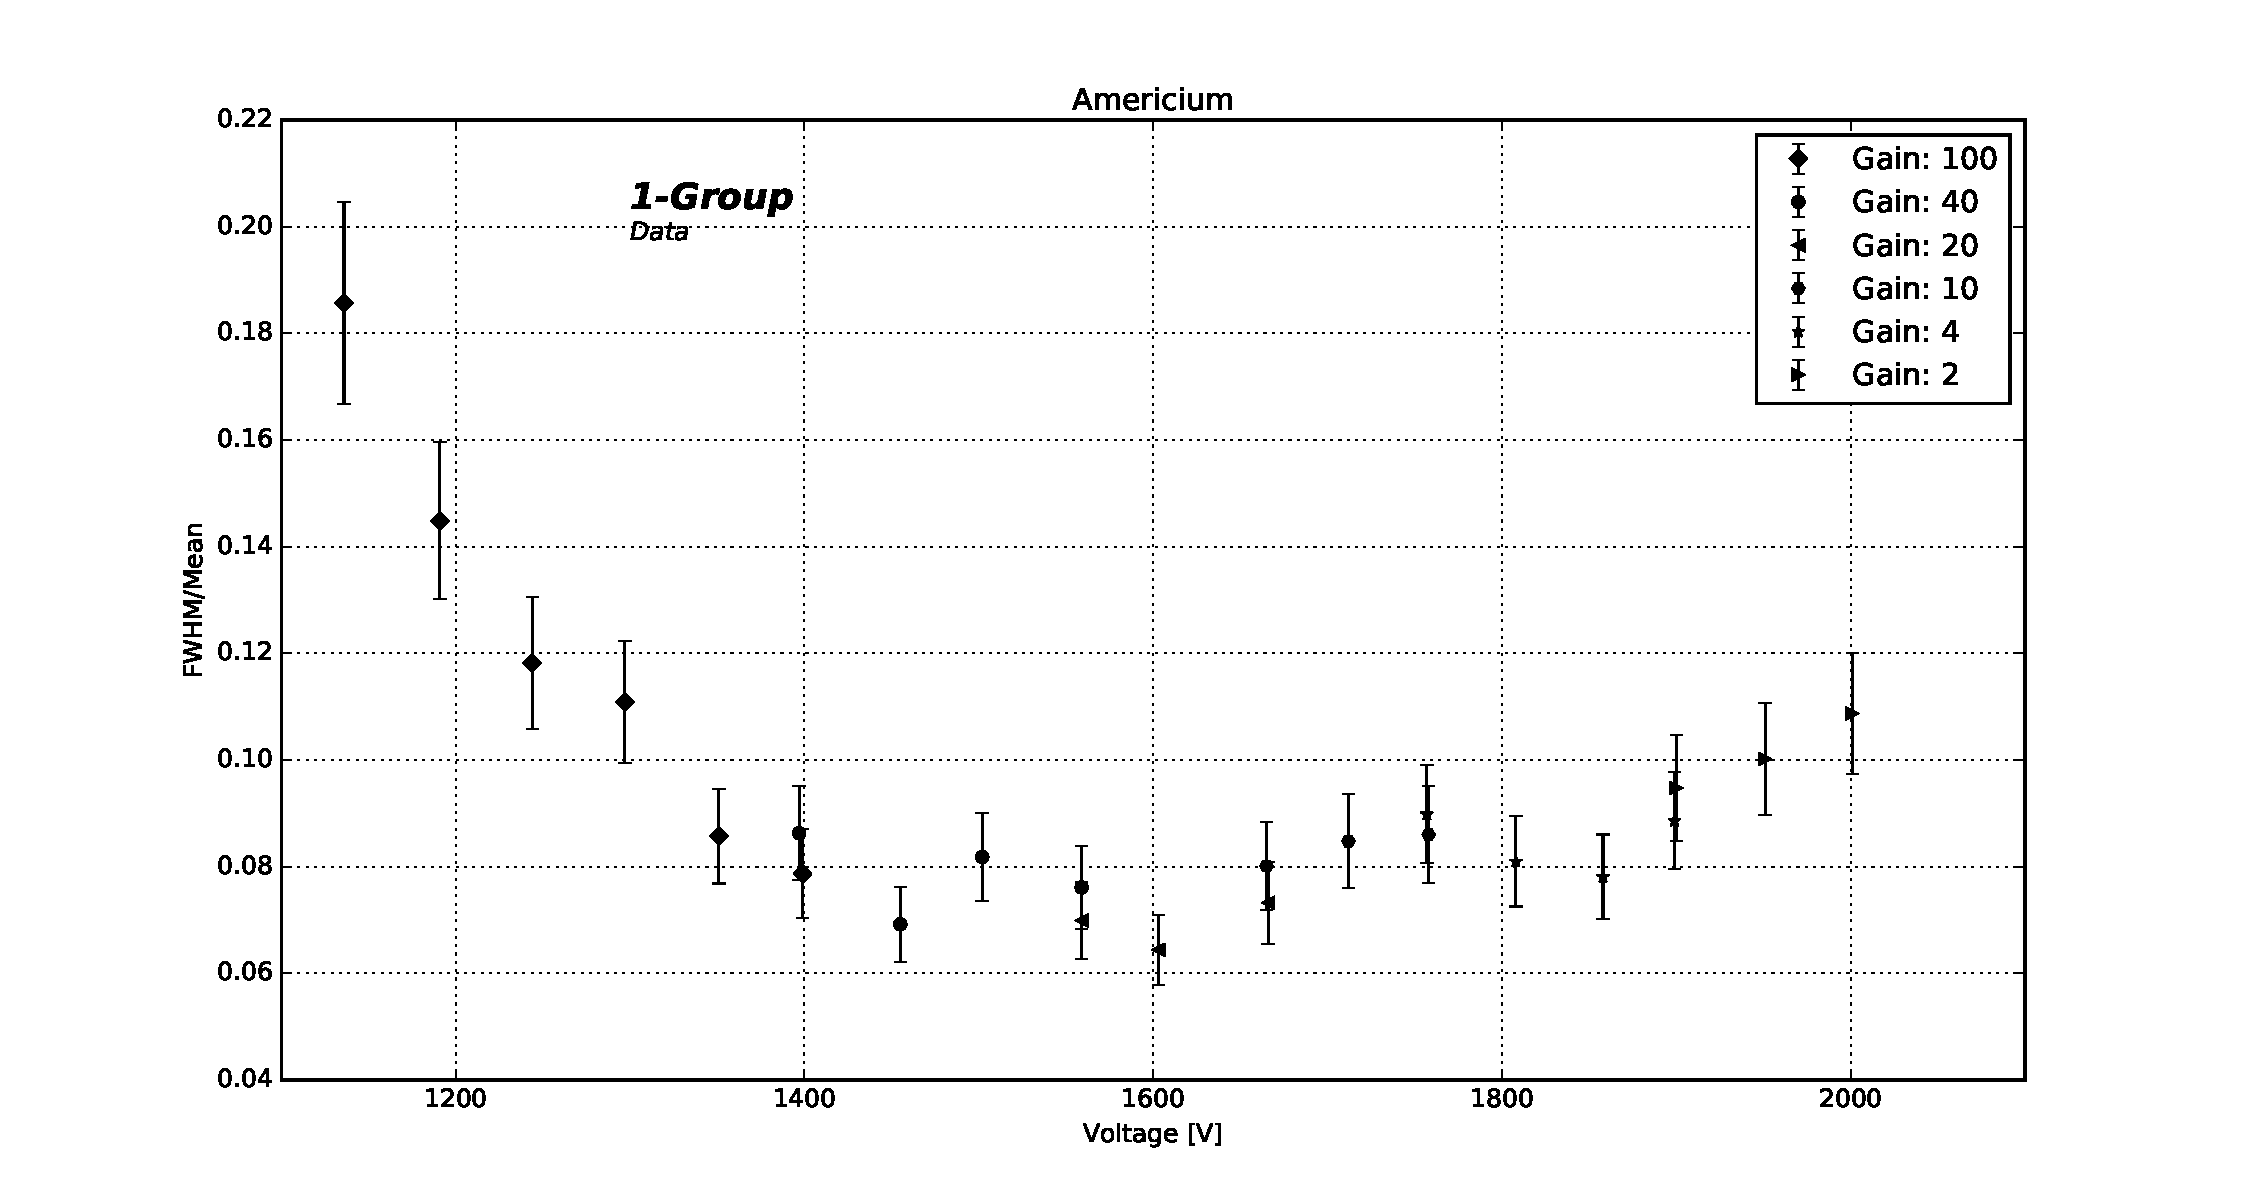
\includegraphics[width=\linewidth]{graphics/americium_scan}
  \caption{Americium scan}
  \label{fig:resolution:americium}
\end{figure*}

\begin{figure*}[htbp]
  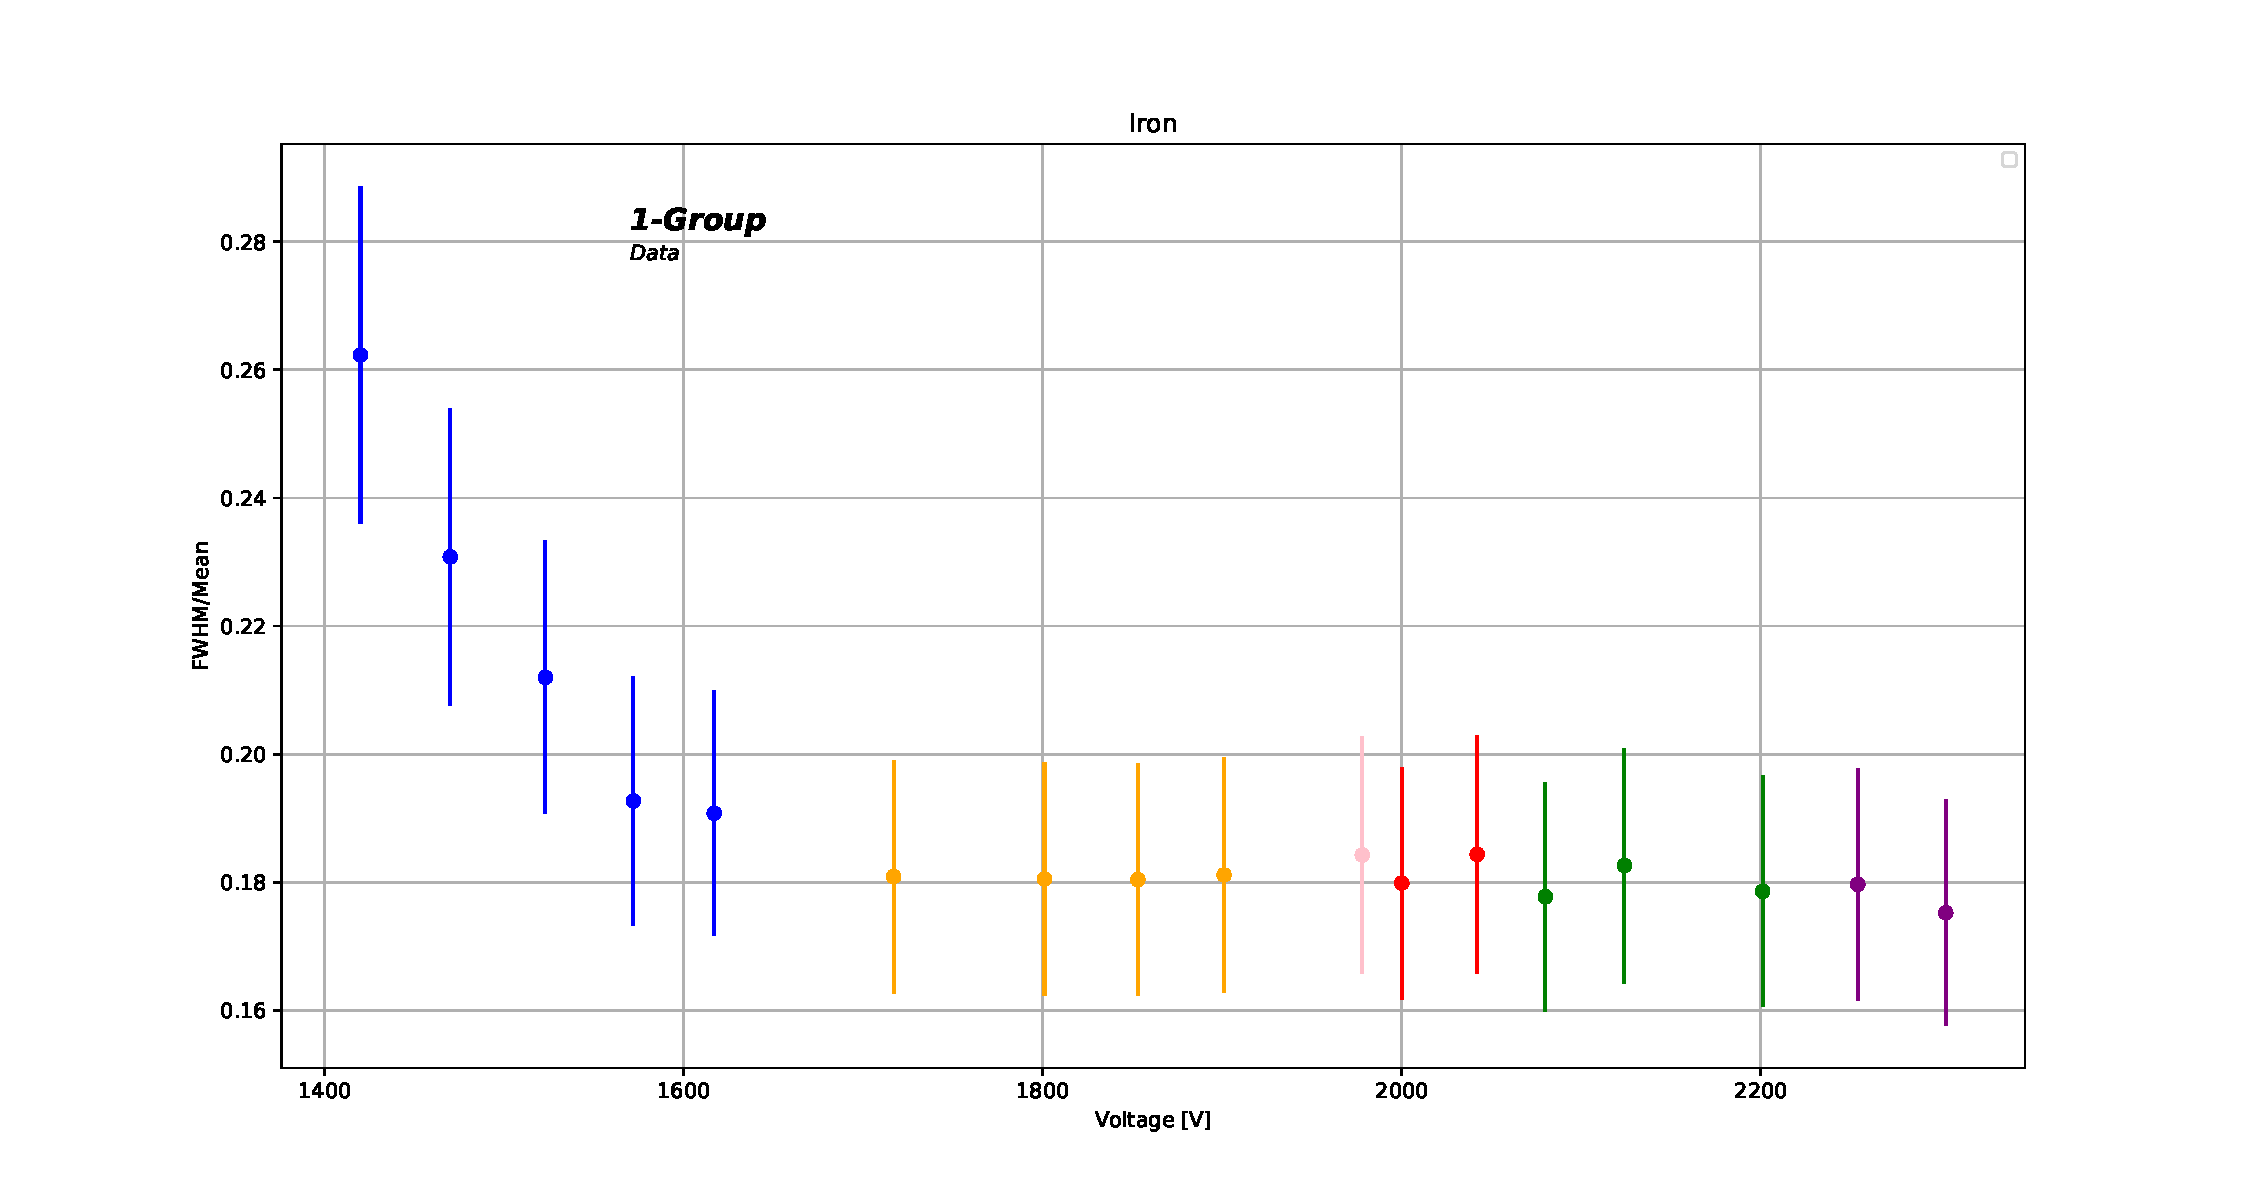
\includegraphics[width=\linewidth]{graphics/iron_scan}
  \caption{Iron scan}
  \label{fig:resolution:iron}
\end{figure*}


%%%%%%%%%%%%%%%%%%%%%%%%%%%%%%%%%%%%%%%%%%%%
% Charge multiplication
%%%%%%%%%%%%%%%%%%%%%%%%%%%%%%%%%%%%%%%%%%%%

\section{Charge Multiplication}
\label{sec:systematics}

In Sect.~\ref{sec:energy_scan} the resolution for each voltage (with its coarse gain) is calculated by finding the FWHM and the mean of the characteristic peak of the two materials.
The same data can be used to calculate the collected charge as a function of the applied voltage. In fact, the MCA mean of the peaks can be converted in an amount of charge using the calibration curve in Fig.~\ref{fig:charge_calibration}. Since the data in Figs.~\ref{fig:resolution:americium} and \ref{fig:resolution:iron} are taken at different coarse gains and the calibration data are collected with coarse gain $10$, a factor needs to be applied to correct for the difference, with the factor being $10/G_\mathrm{coarse}$. For each measurement $i$, then, the collected charge is calculated as such:

\begin{adjustwidth}{-1cm}{}
\begin{align}
Q_{\mathrm{coll}, i} = (b + a \cdot mean_{MCA, i}) \cdot \frac{10}{G_{\mathrm{coarse}, i}} 
\end{align}
\end{adjustwidth}

where $Q_{\mathrm{coll}, i}$ is the collected charge per measurement, $a$ and $b$ are the calibration function parameters from Fig.~\ref{fig:charge_calibration}, $mean_{MCA, i}$ is the mean of the gaussian in the MCA spectrum and $G_{\mathrm{coarse}, i}$ is the coarse gain used for the measurement. In order to obtain the number of electrons, $Q_\mathrm{coll, i}$ is then divided by the charge of one electron $1.602 \cdot 10^{-19}$ C. The results for both Am and Fe are shown in Fig.~\ref{fig:number_of_electrons}, where the errorbars are smaller than the data points. The uncertainties on these points are both statistial and systematics and they are combined in quadrature; in particular, the systematic uncertainties come from the systematic uncertainties on $mean_{MCA, i}$ and on $G_{\mathrm{coarse}, i}$.


\begin{figure}[htb]
  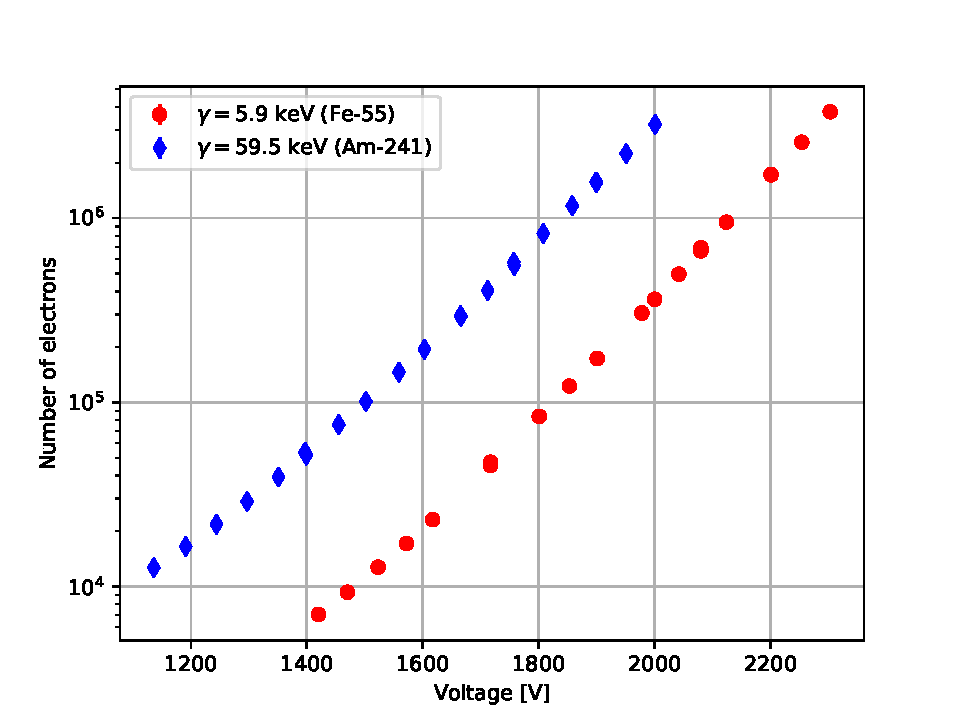
\includegraphics[width=0.5\textwidth]{graphics/numbervsvoltage.pdf}
  \caption{Charge collected in the cider can proportional detector as a function of the voltage applied for the Fe and Am sources. Note that the errorbars are smaller than the plotted points.}
  \label{fig:number_of_electrons}
\end{figure}

After having calculated the number of electrons collected as a function of voltage, we can find the measured multiplication factor per measurement $i$ as

\begin{align}
\label{eq:Mexp}
M_{\mathrm{experimental},i} &= \frac{N_{\mathrm{carriers},\mathrm{out},i}}{N_\mathrm{carriers~per~avalanche}} \nonumber \\
                            &= \frac{Q_{\mathrm{coll},i}}{n_{\mathrm{Fe}^{5},\mathrm{Am}^{241}}\cdot e}
\end{align}

where $M_{\mathrm{experimental},i}$ is the experimentally measured multiplication factor, $Q_{\mathrm{coll},i}$ is the charge collected per measurement, $e$ is the electron charge and $n_{\mathrm{Fe}^{55},\mathrm{Am}^{241}}$ is the average number of electrons-ion pairs produced by either Fe$^{55}$ (227) or Am$^{241}$ (2290), as taken from \cite{can_paper}.

In order to compare those found values with the theoretical expectation, we computed the multiplication factor with the parameters of our experiment (and of the environment the experiment was conducted in) using this formula, which assumes that our detector is operating in the linear regime (\cite{gas_detect}):

\begin{adjustwidth}{+0.5cm}{}
\begin{align}
\ln(M)=\frac{\ln(2)}{\ln(r_{c}/r_{a})}\cdot\frac{V}{\Delta V}\cdot\ln\left[ \frac{V\rho_{o}}{ra\ln(r_{c}/r_{a})E_\mathrm{min}(\rho_{o})\rho}\right]
\label{eq:lnm}
\end{align}
\end{adjustwidth}

The meaning and values associated with each parameter of this equation is listed in Tab.~\ref{Tab:params}. One can see that most of these values either come from tabulated properties of the gas used, or are derived from the initial measurement of the beer can dimensions, listed in Tab.~\ref{Tab:cidercan_sizes} for reference.

\begin{table*}[htb]
  \begin{tabularx}{\linewidth}{p{1.5cm}p{8cm}rl}
    \textbf{Variable}     & \textbf{Definition}                                                         & \textbf{Value}     & \textbf{Source}  \\
    \hline
    $r_{c}$                 & radius of the cathode                                                       & $3.121 \pm 0.003$      & Eq.~\ref{eq:rcra}   \\
    &&&\\
    $r_{a}$                 & radius of the anode                                                         & $\SI{25 +- 2}{\micro\meter}$ & Eq.~\ref{eq:rcra}   \\
    &&&\\
    $V$                    & operating voltage                                                           & 1-3 kV             & N/A                \\
    &&&\\
    $\Delta V$             & potential required to produce an additional electron                & $23.6 \pm 5.4$ V   &\cite{gas_detect}   \\
    &&&\\
    $E_\mathrm{min}(\rho_{o})$      & \begin{tabular}[c]{@{}l@{}}Minimal electric field needed for ionisation\\(at standard pressure)\end{tabular}         & $48. \pm 3$ kV/cm  &\cite{gas_detect}   \\
    &&&\\
    $\rho_{o}/\rho$ & \begin{tabular}[c]{@{}l@{}}Standard density of the gas\\(compared to density at  T=273K and P = 1 bar)\end{tabular}  &                    &Eq.~\ref{eq:gaslaw}, \cite{meteo}\\
    \hline
  \end{tabularx}
  \caption{List of the main systematics sources}
  \label{Tab:params}
\end{table*}

For the geometric properties, the relationship between the measured quantities and the anode radius, is simply $r_{a} = d_{a}/2$, with $d_{a}$ being the radius of the anode wire. Meanwhile, the radii of the cathode is related to the other measurements via Eq.~\ref{eq:rcra}.

\begin{align}
  \label{eq:rcra}
  r_{c} = \frac{D_\mathrm{outer}}{2}-\tau
\end{align}

where $D_\mathrm{outer}$ is the outer radius of the cider can and $\tau$ is the can wall thickness.
To determine the gas properties at the environmental conditions of the laboratory, the temperature and pressure of the room need to be measured. With these values on hand, the ratio of gas densities can be determined by using the ideal gas law.

\begin{align}
  \label{eq:gaslaw}
  \frac{\rho}{\rho_{o}} = \frac{P}{P_{o}}\cdot \frac{T_{o}}{T}
\end{align}

with $\rho$ being the gas density, $P$ the gas pressure and $T$ its temperature.
During the measurements, the temperature stayed mostly constant, but the pressure varied over the course of the day, as shown in Fig.~\ref{fig:pressure}. The uncertainty on the pressure was thus selected to be the largest pressure change with respect to standard pressure, over the course of a day.

\begin{figure}[htb]
  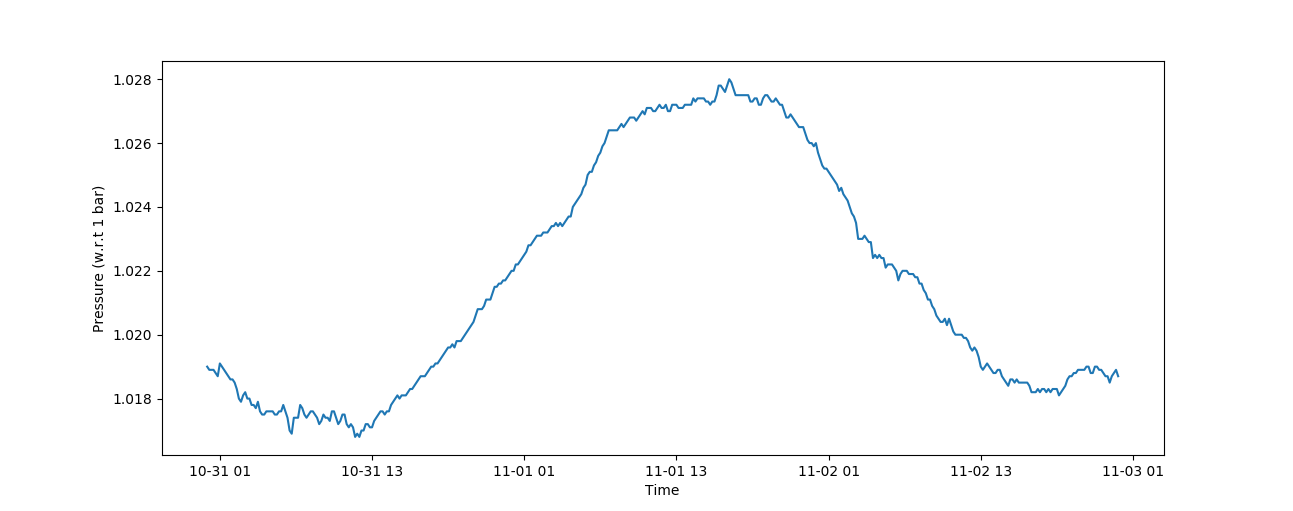
\includegraphics[width=0.5\textwidth]{graphics/pressure_monitoring.png}
  \caption{Atmospheric pressure in Helsinki during the spectra measurement. Source: \cite{meteo}}
  \label{fig:pressure}
\end{figure}

Given the parameters and uncertainties quoted in Tab.~\ref{Tab:params}, a MC simulation was created in order to compute the theoretical uncertainties on the expected multiplication factor as a function of operating voltage. In this systematics treatment, each parameter was drawn out of Gaussian shaped probability distribution, with a mean centred at a parameter's value and the width set as the quoted uncertainty. Fig.~\ref{final_lnm} shows the 1$\sigma$ and 2$\sigma$ confidence interval of the multiplication factor, after propagation of systematic uncertainties.


%The theoretical expectation for the drift chamber's electron yield can be compared to the data obtained during the iron spectrum scan described in Sect.~\ref{sec:resolution_scans}. Given a number of MCA counts $Q_{mca}$, the charge accumulated at the electrodes of the drift chamber can be obtained with Eq.~\ref{eq:M_exp}.

%\begin{align}
%  \label{eq:M_exp}
%  Q_{detector} = \frac{Q_{MCA}}{G_{pre,mca}\cdot{G_{coarse}}}s
%\end{align}

%where $G_{pre,mca}$ is the preamplifier gain in units of $d.c./V$ (as plotted in Fig.~\ref{fig:preamp_gain_mca}),and $G_{coarse}$ is the coarse gain that was described and measured in Sect.~\ref{sec:coarse}. From that point, the multiplication factor of the experimental data is given by Eq.~\ref{eq:Mexp}.

%\begin{align}
%  \label{eq:Mexp}
%  M_{experimental} &= \frac{N_{carriers,out}}{N_{carriers per avalanche}} \nonumber \\
%                   &= \frac{Q_{detector}}{n_{Fe^{5},Am^{241}}\cdot e}
%\end{align}

%Where $n_{Fe^{55},Am^{241}}$ is the average number of electrons-ion pairs produced by either Fe$^{55}$ (227) or Am$^{241}$ (2290), as taken from \cite{can_paper}. 

The measured multiplication factors obtained in each voltage scan is shown in Fig.~\ref{final_lnm}, along with the theoretical expectation for their values given the geometry of the can detector and the environmental conditions during the measurement. As one can see, the data collected lies within the $1\sigma$ band of the theoretically predicted values.

\begin{figure}[htb]
  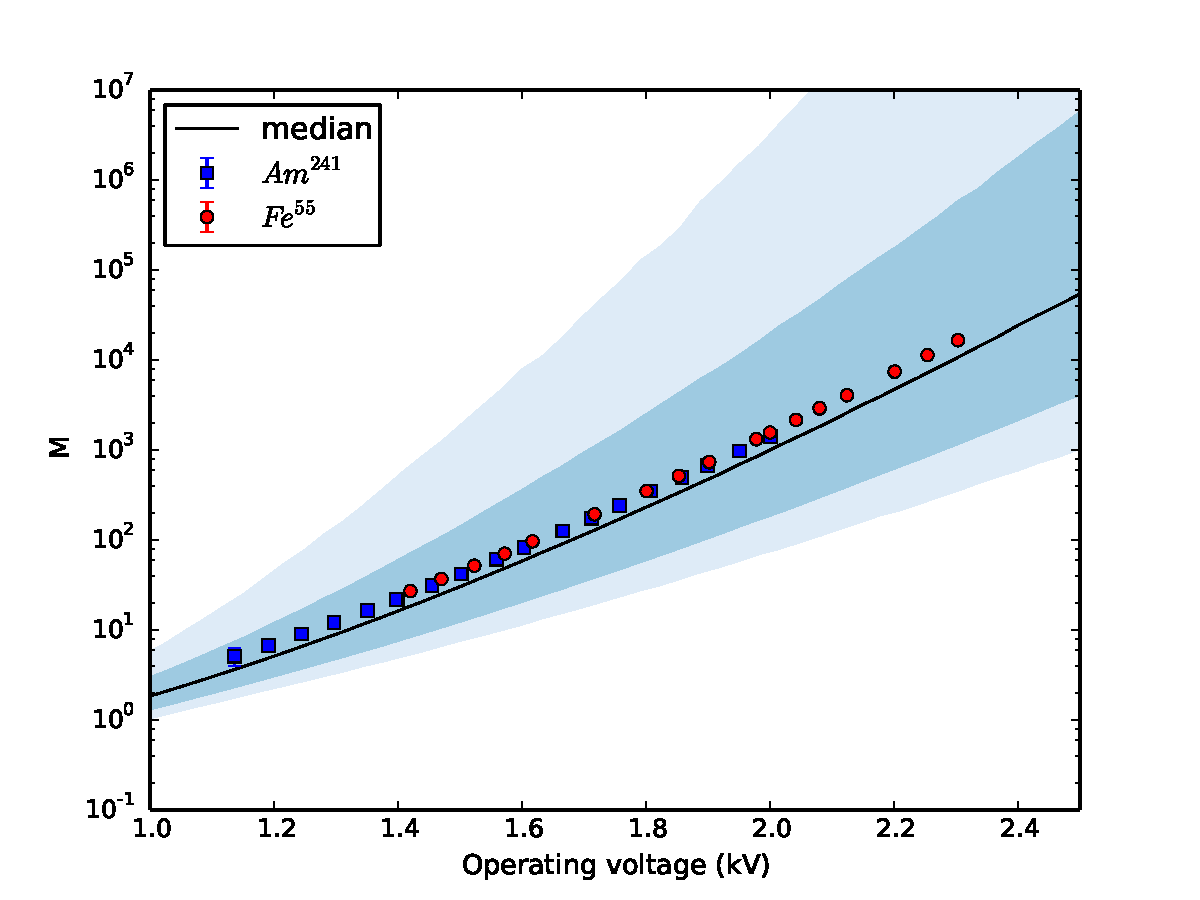
\includegraphics[width=0.55\textwidth]{graphics/lnM_final_plot_new.pdf}
  \caption{Natural logarithm of the drift chamber's multiplication factor M. Red and green data points represent the results obtained with Fe$^{55}$ and Am$^{241}$ respectively. Blue bands show the theoretical expectation for the detector, given systematics uncertainties in the cider can geometry and gas properties.}
  \label{final_lnm}
\end{figure}

\FloatBarrier